\section{Fiche de la Thailande}

Date: 30/05/2008

\begin{multicols}{2}

\textbf{\textsc{Drapeau}}

\hspace*{-0.65cm}
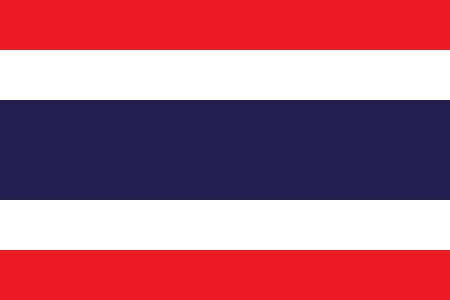
\includegraphics[width=4.8cm]{articles/Fiche-de-la-thailande/drapeau_thailande.png}
Drapeau de la Thaïlande.

\textbf{\textsc{Situation}}

D’une superficie de 513.115 km2, sensiblement égale a la France, la Thailande s’etend du 5e au 21e parallele, soit sur pres de 1.770 km de long ; sa plus grande largeur d’est en ouest est de 805 km mais se reduit a 50 km a la hauteur de l’isthme de Kra.
Elle est limitée a l’est et au nord-est par le Laos, au sud-est par le Cambodge, au sud par la Malaisie, au nord-ouest et a l’ouest par la Birmanie. On distingue cinq regions principales :

La région centrale, vaste plaine alluviale du Menam Chao Phraya, le plus grand fleuve thailandais. Cette plaine bien arrosee et iriguee, constituee de riches sediments, est a la fois le grenier a riz du pays, son centre historique avec Bangkok, industriel, urbain et financier. Elle est bordee a l’est par le Cambodge et donne au sud sur le golfe de Thailande. C’est la region la plus peuplee.

La région montagneuse du nord et de l’ouest, qui longe la frontiere birmane et culmine au mont Doi Inthanon (2 595 m), peu peuplee, recouverte de forets.

La région est ou s’etend un plateau greseux aride, le plateau du Korat, bordant la vallee du Mekong, qui separe la Thailande du Laos. La region nord-est est une region pauvre et rurale, avec de petites exploitations qui ne supportent plus qu’une recolte annuelle. 15\% des terres sont cultivees et l’elevage du gros betail est dominant. Les importants travaux d’irrigation n’ont pas eu les retombees esperees.

La région sud-est comprend les massifs de Dongrek et de Khao Khieu qui delimitent la frontiere avec le Cambodge ;

Le sud, situe sur la presqu’ile de Malacca est borde a l’ouest par la Birmanie et la mer d’Andaman. Cette region, soumise a la mousson, est tres arrosee. A l’est on trouve le golfe de Thailande et au sud la Malaisie. Cette zone bien arrosee produit le riz, l’hevea, pratique la peche et dispose aussi de ressources minieres (zinc).

\textbf{\textsc{Population}}

80\% des Thaïlandais sont des Thaïs, un ensemble de peuples originaires de la Chine occidentale. Les Chinois constituent la minorité la plus importante, environ 10\% de la population. Parmi les autres minorités figurent les musulmans (1,5 million) d’origine malaise qui vivent dans le Sud, les "tribus" montagnardes du nord (Karens, Hmongs, Akhas, Lahus), les réfugiés Viêtnamiens et Cambodgiens (Khmers) et une importante population de travailleurs Birmans "clandestins" (environ 800.000).

|                                       |     THAILANDE   |    FRANCE    |
| ------------------------------------- |: -------------: | -----------: |
|Population                             |    61,2 millions| 59,2 millions|
|Densite                                |      118 hab.km2|   108 hab.km2|
|Accroissement naturel de la population |              1,1|           0,4|
|Indice de fecondite                    |             1,87|           1,8|
|Esperance de vie                       |           69 ans|      78,5 ans|
|Urbanisation                           |           43,3 \%|        75,6 \%|

\textbf{\textsc{Climat}}

Le climat de la Thaïlande est tropical et humide. On distingue trois saisons :
- une saison sèche très chaude (mars - juin)
- une saison des pluies (juillet - octobre)
- une saison plus fraîche (novembre - février).
On note de grandes variations climatiques en fonction des regions. Dans l’ensemble l’amplitude thermique est faible en Thaïlande. Les températures moyennes mensuelles à Bangkok varient entre 31 et 35 degrés C sur l’année. Le degré hygrométrique varie de 45 a 85\%.

\textbf{\textsc{Villes principales}}

\textbf{Bangkok}
Capitale et plus grande ville du royaume (8 millions d’habitants, 12 millions avec la banlieue), située au centre du pays, sur les rives du Menam Chao Phraya, près du golfe de Siam. Bangkok est un des grands carrefours commerciaux du Sud-Est asiatique et un important port de transit qui assure la majorité des échanges exterieurs du pays. La ville, située dans une région productrice de riz, est aussi le premier centre industriel du pays (agro-alimentaire, textile, ciment, pétrole raffine et constructions mécaniques). La ville est le siège du Comité économique et social des Nations unies pour l’Asie et le Pacifique ainsi que de l’Organisation du traité de l’Asie du Sud-Est (OTASE). Centre de la culture et de l’enseignement thaï, Bangkok compte plusieurs universités et collèges techniques. On peut y admirer quelques 400 temples somptueusement décorés (les wats) dont le Wat Phra Kaeo (Temple du boudha d’émeraude) situé à l’intérieur des murs du Grand Palais. Elle est parcourue de très nombreux canaux et les marchés flottants, où les embarcations servent de lieux de vente, sont encore très actifs. La ville est tres polluée et est connue pour ses embouteillages légendaires.

\textbf{Chiang Mai}
Située à environ 720 km au nord de Bangkok et à 130 km de la frontière avec la Birmanie, sur la rivière Ping, la ville est le grand centre économique du nord de la Thailande (500.000 habitants) ainsi qu’un terminus ferroviaire. La ville ancienne conserve les vestiges de temples datant du 13ème et 15ème siècles, dont celui du Wat Phra Dhat Doi Suthep censé abriter les reliques de Bouddha. Outre le tourisme, la ville vit du commerce du teck, de ses productions agricoles et de ses objets artisanaux (laques, poteries, produits de luxe).

\textbf{Nakhon Ratchasima}
Située au Nord-Est du pays, à 256 km de Bangkok, sur le fleuve Moun, dans la partie méridionale du plateau de Khorat. La ville compte 204.000 habitants. C’est un centre industriel (matériel ferroviaire, agroalimentaire, tissages) et commercial mais également un centre universitaire et l’un des hauts lieux du bouddhisme.

\end{multicols}

\vfill
